% ============================================================
% Estado del Arte -- Practicum 2.2 -- UTPL 2026
% Formato IEEE Conference (IEEEtran)
% ============================================================

\documentclass[10pt,twocolumn,spanish]{IEEEtran}

% ── paquetes ──────────────────────────────────────────────────────────────────
\usepackage[T1]{fontenc}
\usepackage[utf8]{inputenc}
\usepackage[spanish,es-nodecimaldot]{babel}
\usepackage{cite}
\usepackage{amsmath,amssymb}
\usepackage{graphicx}
\usepackage{url}
\usepackage{hyperref}
\usepackage{booktabs}
\usepackage{array}
\usepackage{tabularx}
\usepackage[table]{xcolor}
\usepackage{microtype}

% ── colores IEEE ──────────────────────────────────────────────────────────────
\definecolor{ieeehead}{gray}{0.20}
\definecolor{ieeegray}{gray}{0.92}

% ── columna con alineacion izquierda ─────────────────────────────────────────
\newcolumntype{L}[1]{>{\raggedright\arraybackslash}p{#1}}

% ── hiperlinks ────────────────────────────────────────────────────────────────
\hypersetup{
  colorlinks=true,
  linkcolor=black,
  citecolor=black,
  urlcolor=blue,
  breaklinks=true
}

% ── placeholder de imagen ─────────────────────────────────────────────────────
\newcommand{\imgplaceholder}[2]{%
  \vspace{4pt}%
  \noindent\fbox{%
    \begin{minipage}[c][#2][c]{\dimexpr\columnwidth-2\fboxsep-2\fboxrule\relax}
      \centering
      \textbf{#1}\\[6pt]
      \small\textit{Inserta tu imagen exportada desde draw.io}
    \end{minipage}%
  }%
  \vspace{4pt}%
}

% =============================================================================
\begin{document}

\title{Pipeline de Datos del Macroentorno Ecuatoriano:\\
Limpieza, Modelo Relacional y Dashboard Analitico}

\author{
  \IEEEauthorblockN{Martin Emanuel Ruiz Sanchez}
  \IEEEauthorblockA{
    Carrera de Computacion\\
    Universidad Tecnica Particular de Loja\\
    Loja, Ecuador\\
    meruiz22@utpl.edu.ec
  }
}

\maketitle

% ── abstract ─────────────────────────────────────────────────────────────────
\begin{abstract}

\end{abstract}

\begin{IEEEkeywords}

\end{IEEEkeywords}

% =============================================================================
\section{Introduccion}

El Tablero Macroentorno de la UTPL consolida indicadores economicos
y laborales de nueve fuentes publicas del Ecuador.
Su actualizacion es manual y su pipeline carece de documentacion
reproducible.
Cuando cambia un archivo fuente, el conocimiento para actualizarlo
vive en personas, no en codigo.

El reto de Practicum~2.2 de 6to ciclo resuelve ese problema en
siete semanas.
El pipeline parte de los archivos crudos que entrega el equipo de RPA
y termina en un dashboard con tres preguntas analiticas respondidas.
El stack es Python, PostgreSQL y Power~BI.

El dashboard responde tres preguntas concretas para la UTPL.
P1 analiza la evolucion economica ecuatoriana de los ultimos
20 anos con datos del BCE.
P2 identifica los sectores y provincias con mayor actividad
economica y empleo usando VAB, ENEMDU y el Censo 2022.
P3 cruza bachilleres por provincia (MINEDUC) con empresas
activas (Supercias) para detectar zonas con demanda potencial
de educacion superior; ese cruce alimenta directamente el
Tablero de Segmentacion de Marketing de la UTPL.

Construir ese pipeline requiere competencias que el mercado
demanda con urgencia.
El Future of Jobs Report 2025 proyecta que la demanda de
especialistas en Big~Data crece mas del 100\% entre 2025
y 2030~\cite{wef2025}.
La UTPL forma a esos especialistas con datos reales,
fuentes publicas y decisiones tecnicas concretas.

El estado del arte responde cuatro preguntas vinculadas a los
entregables del reto:
\begin{itemize}
  \item \textbf{P1.} Que arquitectura integra fuentes heterogeneas
        de datos publicos en un pipeline reproducible.
  \item \textbf{P2.} Como se disena el modelo relacional antes de
        escribir codigo.
  \item \textbf{P3.} Que stack tecnico y practicas de limpieza son
        criticos para cargar fuentes heterogeneas correctamente.
  \item \textbf{P4.} Como se integra el pipeline con un proceso de
        automatizacion y que anticipa ese patron para 2025--2030.
\end{itemize}

% =============================================================================
\section{Marco Conceptual}

\textbf{Data Warehouse.}
Repositorio central de datos historicos estructurados, integrados desde
multiples fuentes y optimizados para consultas
analiticas~\cite{kimball2013}.
Transforma los datos antes de cargarlos (ETL) y mantiene esquemas fijos.

\textbf{Data Lake.}
Almacen de datos en formato crudo sobre almacenamiento de objetos de
bajo costo~\cite{sawadogo2021}.
Acepta datos estructurados, semi-estructurados y no estructurados sin
transformacion previa.
Requiere metadatos activos para mantener la rastreabilidad de cada
archivo.

\textbf{Data Lakehouse.}
Arquitectura que une la flexibilidad del Data Lake con las garantias
transaccionales del Data Warehouse en una sola
plataforma~\cite{armbrust2021}.
Soporta cargas analiticas y de machine learning sin mover datos entre
sistemas.

\textbf{Arquitectura Medallon (Bronze--Silver--Gold).}
Patron de tres zonas de calidad progresiva dentro de un
Lakehouse~\cite{databricks2024}.
Bronze guarda los datos en su estado original e inmutable.
Silver aplica limpieza, tipado y normalizacion.
Gold materializa vistas o tablas derivadas listas para el dashboard.
En el reto, Bronze recibe los archivos de RPA, Silver los almacena en
PostgreSQL con doce tablas y FK correctas, y Gold expone cuatro vistas
para Power~BI.

\textbf{ETL (Extract, Transform, Load).}
Proceso que extrae datos, los transforma en un motor intermedio y los
carga ya limpios en el destino~\cite{kimball2013}.
Es el patron clasico del Data Warehouse.

\textbf{ELT (Extract, Load, Transform).}
Variante que carga los datos en crudo primero y transforma dentro del
motor de destino~\cite{machado2022}.
El reto sigue ELT: cada modulo Python carga en PostgreSQL y las vistas
Gold transforman ahi mismo.

\textbf{Pipeline de datos.}
Secuencia automatizada de pasos que mueve y transforma datos desde
las fuentes hasta el destino~\cite{naso2024}.
El pipeline del reto es reproducible: \texttt{pipeline.py} detecta
archivos nuevos de RPA y los procesa sin intervencion manual.

\textbf{Modelo Entidad-Relacion (ER).}
Representacion grafica de entidades, atributos y relaciones de un
dominio~\cite{barret2025}.
El diagrama ER del reto define \texttt{dim\_tiempo} y
\texttt{dim\_geografia} como dimensiones compartidas entre las nueve
fuentes, y especifica las claves foraneas de cada tabla \texttt{fact\_}
antes de escribir codigo.

% =============================================================================
\section{Trabajos Relacionados}

La Tabla~\ref{tab:related} sintetiza los trabajos que fundamentan
las decisiones tecnicas del reto.

\begin{table}[ht]
\caption{Trabajos relacionados}
\label{tab:related}
\renewcommand{\arraystretch}{1.2}
\footnotesize
\begin{tabularx}{\columnwidth}{L{1.4cm} L{2.1cm} L{3.8cm}}
\toprule
\rowcolor{ieeehead}
\textcolor{white}{\textbf{Ref.}} &
\textcolor{white}{\textbf{Aporte}} &
\textcolor{white}{\textbf{Conexion directa con el reto}} \\
\midrule
\rowcolor{ieeegray}
\cite{armbrust2021} &
Formaliza el Lakehouse: storage y ACID &
Bronze recibe archivos de RPA. Silver en PostgreSQL aplica ACID. \\
%
\cite{sawadogo2021} &
Sin linaje el repositorio se degrada &
Cada modulo documenta sus decisiones de limpieza: nulos, tipos y
deduplicacion. \\
%
\rowcolor{ieeegray}
\cite{kimball2013} &
Metodologia dimensional de 4 pasos &
Define \texttt{dim\_tiempo}, \texttt{dim\_geografia} y las doce
tablas Silver con FK. \\
%
\cite{machado2022} &
ELT: cada fuente propietaria de su logica &
\texttt{bce.py}, \texttt{inec.py}, \texttt{supercias.py} y
\texttt{mineduc.py} encapsulan la limpieza de su fuente. \\
%
\rowcolor{ieeegray}
\cite{bhardwaj2024} &
RPA optimiza ingestion; contratos criticos &
El acuerdo de semana~4 fija subcarpeta, formato de nombre y canal
de notificacion. \\
%
\cite{barret2025} &
Grafos ER son el estandar de BD modernas &
El tutor aprueba el diagrama ER en semana~1 (10\% evaluacion) antes
de que el estudiante escriba codigo. \\
%
\rowcolor{ieeegray}
\cite{tadakala2025} &
Parrafo interpretativo supera a la estetica &
6to ciclo exige un parrafo de analisis ejecutivo por pagina del
dashboard. \\
%
\cite{lai2025} &
Preparacion de datos consume $>$70\% del tiempo &
Las semanas~1 a~4 se dedican a limpieza y modelo. Power~BI se conecta
en semana~5. \\
\bottomrule
\end{tabularx}
\end{table}

Armbrust et al.~\cite{armbrust2021} formalizaron el Lakehouse en
CIDR~2021.
Jain et al.~\cite{jain2023} compararon Delta~Lake, Hudi e Iceberg:
Delta~Lake lidera en velocidad de carga; Iceberg ofrece mayor
interoperabilidad.
Sawadogo y Darmont~\cite{sawadogo2021} confirman que documentar el
linaje de cada archivo es lo que separa un Data Lake util de uno
inutilizable.
Kimball y Ross~\cite{kimball2013} formalizan la metodologia dimensional.
Barret et al.~\cite{barret2025} confirman que el diagrama~ER sigue
siendo la herramienta estandar para comunicar un diseno relacional
antes de implementarlo.
Machado et al.~\cite{machado2022} describen el paso de ETL a ELT en
el contexto Data~Mesh: cada fuente es propietaria de su logica de
limpieza.
Bhardwaj et al.~\cite{bhardwaj2024} demuestran que RPA escala el
procesamiento de datos estructurados cuando los contratos de interfaz
son precisos.
Lai et al.~\cite{lai2025} miden que la preparacion de datos consume
mas del 70\% del tiempo en proyectos de BI.
Tadakala et al.~\cite{tadakala2025} demuestran que los dashboards con
parrafo interpretativo por pagina superan en efectividad a los que
priorizan la presentacion visual.

% =============================================================================
\section{Herramientas y Stack Tecnico}

El reto define un stack de tres capas: Python transforma, PostgreSQL
almacena y Power~BI visualiza.

La Fig.~\ref{fig:er} presenta el modelo~ER.
Se diseña y entrega, antes de escribir
cualquier linea de codigo.
El diagrama muestra las doce tablas con sus claves primarias y foraneas.
\texttt{dim\_tiempo} y \texttt{dim\_geografia} se comparten entre las
nueve fuentes.
Las tablas de hechos (\texttt{fact\_macro\_anual},
\texttt{fact\_empleo}, \texttt{fact\_indicadores\_diarios} y las de
VAB, IEE, Supercias y MINEDUC) referencian esas dimensiones con FK.

\begin{figure}[ht]
  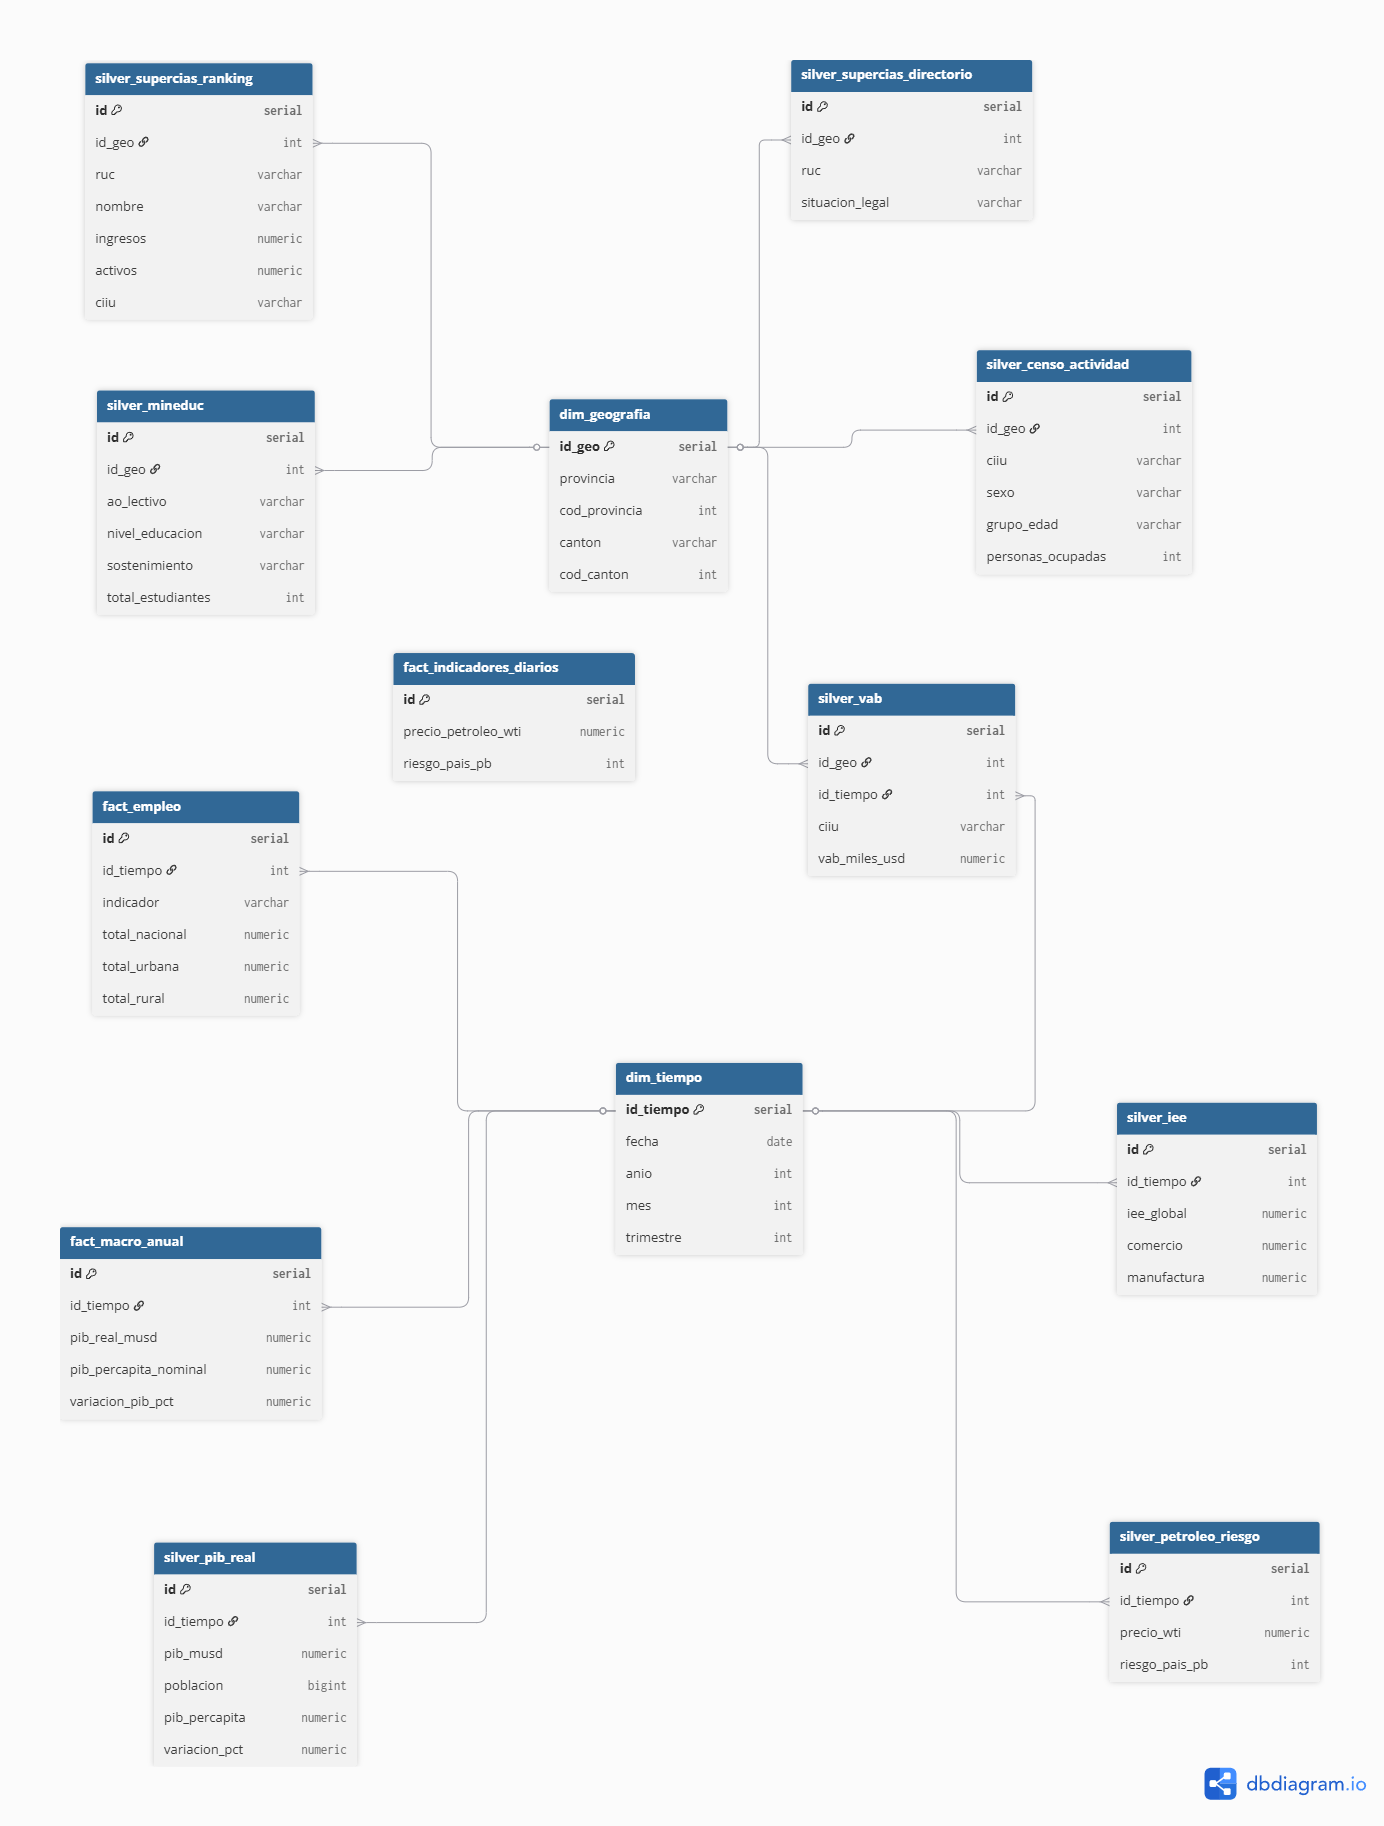
\includegraphics[width=\columnwidth]{modelo_er_silver.png}
  %%\imgplaceholder{Modelo ER -- Capa Silver (PostgreSQL)}{4.6cm}
  \caption{Modelo entidad-relacion de la capa Silver del reto.
    \texttt{dim\_tiempo} y \texttt{dim\_geografia} son dimensiones
    compartidas. Cada tabla \texttt{fact\_} referencia ambas con FK.}
  \label{fig:er}
\end{figure}

La Tabla~\ref{tab:stack} detalla el rol de cada herramienta en el
pipeline.

\begin{table}[ht]
\caption{Stack tecnico del reto de 6to ciclo}
\label{tab:stack}
\renewcommand{\arraystretch}{1.2}
\footnotesize
\begin{tabularx}{\columnwidth}{L{1.5cm} L{1.1cm} L{1.9cm} X}
\toprule
\rowcolor{ieeehead}
\textcolor{white}{\textbf{Herramienta}} &
\textcolor{white}{\textbf{Capa}} &
\textcolor{white}{\textbf{Uso en el reto}} &
\textcolor{white}{\textbf{Tendencia 2025-26}} \\
\midrule
\rowcolor{ieeegray}
Python + pandas &
Bronze a Silver &
\texttt{bce.py}, \texttt{inec.py} (con \texttt{melt()}),
\texttt{supercias.py}, \texttt{mineduc.py} (latin-1) &
polars supera a pandas en velocidad para tablas grandes \\
%
PostgreSQL~16 &
Silver + Gold &
12 tablas Silver con FK. 4 vistas Gold. Vistas materializadas. &
JSONB y particionamiento amplian su rol como capa Silver \\
%
\rowcolor{ieeegray}
Power BI Desktop &
Gold a Dashboard &
DirectQuery a PostgreSQL. Tres paginas: P1, P2 y P3. &
Copilot~IA genera parrafos de analisis en lenguaje natural \\
%
GitHub (privado) &
Versiones &
Modulos ETL, DDL~SQL, README, acuerdo RPA-Datos &
GitHub~Actions valida esquemas en cada commit \\
%
\rowcolor{ieeegray}
draw.io &
Diagrama &
Arquitectura y ER (entregable semana~1) &
Exportacion PDF/PNG para el repositorio \\
\bottomrule
\end{tabularx}
\end{table}

Python procesa cada fuente con un modulo independiente.
\texttt{inec.py} aplica \texttt{melt()} para normalizar la estructura
pivotada de ENEMDU.
\texttt{mineduc.py} lee el AMIE con \texttt{encoding=latin-1} y
separador \texttt{;}, y filtra por bachillerato de ultimo grado.
\texttt{bce.py} convierte las fechas del IEE con
\texttt{pd.to\_datetime()} y carga los cinco archivos del BCE.
PostgreSQL recibe las doce tablas Silver con FK correctas y expone
cuatro vistas Gold.
Power~BI conecta esas vistas via DirectQuery y construye las tres
paginas del dashboard.

% =============================================================================
\section{Tendencias y Futuro}

La Tabla~\ref{tab:tendencias} conecta cinco tendencias del campo de
datos con los entregables especificos del reto.

\begin{table}[ht]
\caption{Tendencias 2025--2030 y conexion con el reto}
\label{tab:tendencias}
\renewcommand{\arraystretch}{1.2}
\footnotesize
\begin{tabularx}{\columnwidth}{L{1.4cm} L{2.0cm} L{3.9cm}}
\toprule
\rowcolor{ieeehead}
\textcolor{white}{\textbf{Tendencia}} &
\textcolor{white}{\textbf{Descripcion}} &
\textcolor{white}{\textbf{Conexion con el reto}} \\
\midrule
\rowcolor{ieeegray}
IA Generativa en pipelines &
Automatiza limpieza e imputacion~\cite{lai2025} &
El reto entrena al estudiante en las decisiones que la IA asistira.
El juicio sobre nulos y tipos de dato en ENEMDU no se delega. \\
%
DataOps continuo &
Pruebas de calidad dentro del pipeline, no despues~\cite{munappy2021} &
El 25\% de evaluacion en tablas Silver correctas replica este principio:
la calidad es criterio de entrega. \\
%
\rowcolor{ieeegray}
Convergencia RPA-Datos &
RPA ingesta fuentes sin API; el contrato de interfaz es el
punto critico~\cite{bhardwaj2024} &
El acuerdo de semana~4 define subcarpeta, formato
\texttt{fuente\_YYYYMMDD.xlsx} y canal de notificacion. \\
%
Data Mesh &
Cada fuente es un producto de dato con propietario y
SLA~\cite{machado2022} &
BCE, INEC, Supercias y MINEDUC son cuatro dominios independientes.
Cada modulo Python es el propietario de su limpieza. \\
%
\rowcolor{ieeegray}
Dashboards con analisis ejecutivo &
Parrafo interpretativo supera al visual puro~\cite{tadakala2025} &
6to ciclo exige un parrafo por pagina que conecte el dato con
la estrategia de la UTPL. \\
\bottomrule
\end{tabularx}
\end{table}

La IA~Generativa automatiza partes de la limpieza, pero la
decision de como normalizar ENEMDU con \texttt{melt()} o como tratar
el primer anio de variacion nula del PIB real requiere juicio del
estudiante~\cite{wef2025}.
DataOps convierte la calidad de dato en parte del flujo de
entrega~\cite{munappy2021}.
El WEF proyecta mas del 100\% de crecimiento en demanda de especialistas
en datos para 2030~\cite{wef2025}.
Las habilidades que el reto desarrolla, diseno ER, limpieza de fuentes
reales y storytelling analitico, son las que el mercado demanda.

% =============================================================================
\section{Conclusiones}

\subsection{P1. Arquitectura para integrar fuentes heterogeneas
en un pipeline reproducible}

La arquitectura Lakehouse con patron medallon Bronze--Silver--Gold
organiza el pipeline en tres zonas de calidad
progresiva~\cite{armbrust2021,databricks2024}
(Fig.~\ref{fig:arquitectura}).
Bronze recibe los archivos de las fuentes publicas sin modificarlos.
Python los transforma y los carga en tablas relacionales en PostgreSQL.
Las vistas Gold alimentan Power~BI con indicadores listos para
el dashboard.
El repositorio GitHub con modulos versionados garantiza que cualquier
miembro del equipo reproduce el resultado.
Sawadogo y Darmont~\cite{sawadogo2021} confirman que documentar el
linaje de cada decision de limpieza es lo que diferencia un
repositorio util de uno inutilizable.

\subsection{P2. Modelo relacional disenado antes de escribir codigo}

Kimball y Ross~\cite{kimball2013} proveen el marco de cuatro pasos:
proceso de negocio, granularidad, dimensiones y metricas.
El esquema resultante tiene dimensiones compartidas entre las fuentes
y tablas de hechos con FK correctas (Fig.~\ref{fig:er}).
Barret et al.~\cite{barret2025} confirman que el diagrama~ER comunica
el diseno antes de que el codigo exista.
El tutor aprueba ese diagrama al inicio del proyecto.
Cada error detectado en el diagrama es un error que no aparece
en la base de datos.

\subsection{P3. Stack tecnico y practicas de limpieza para fuentes
heterogeneas}

Python procesa cada fuente con un modulo independiente que encapsula
su logica de limpieza: renombrado de columnas, tratamiento de nulos,
conversion de tipos y normalizacion de fechas.
PostgreSQL almacena las tablas relacionales y expone vistas Gold
listas para DirectQuery.
Power~BI construye tres paginas analiticas que responden las preguntas
P1, P2 y P3 del dashboard.
Lai et al.~\cite{lai2025} miden que mas del 70\% del tiempo de un
proyecto de BI va a preparacion de datos.
Dedicar la mayor parte del trabajo a la limpieza y al modelo antes
de conectar la herramienta de visualizacion es la practica que
distingue proyectos de BI exitosos de los que fallan en produccion.

\subsection{P4. Integracion con automatizacion y perspectiva 2025-2030}

La integracion entre el pipeline de datos y un proceso de
automatizacion requiere un contrato de interfaz preciso: nombre de
carpeta, formato de archivo y canal de notificacion.
Bhardwaj et al.~\cite{bhardwaj2024} demuestran que la automatizacion
escala cuando esos contratos son precisos.
El pipeline detecta los archivos nuevos y los procesa sin
intervencion manual (Fig.~\ref{fig:arquitectura}).
Para 2030, el Data~Mesh y DataOps consolidan un modelo donde cada
fuente es un producto de dato con propietario y SLA~\cite{machado2022}.
El estudiante que termina este reto practica ese modelo con datos
reales desde el primer dia.

% =============================================================================
\begin{figure}[t]
  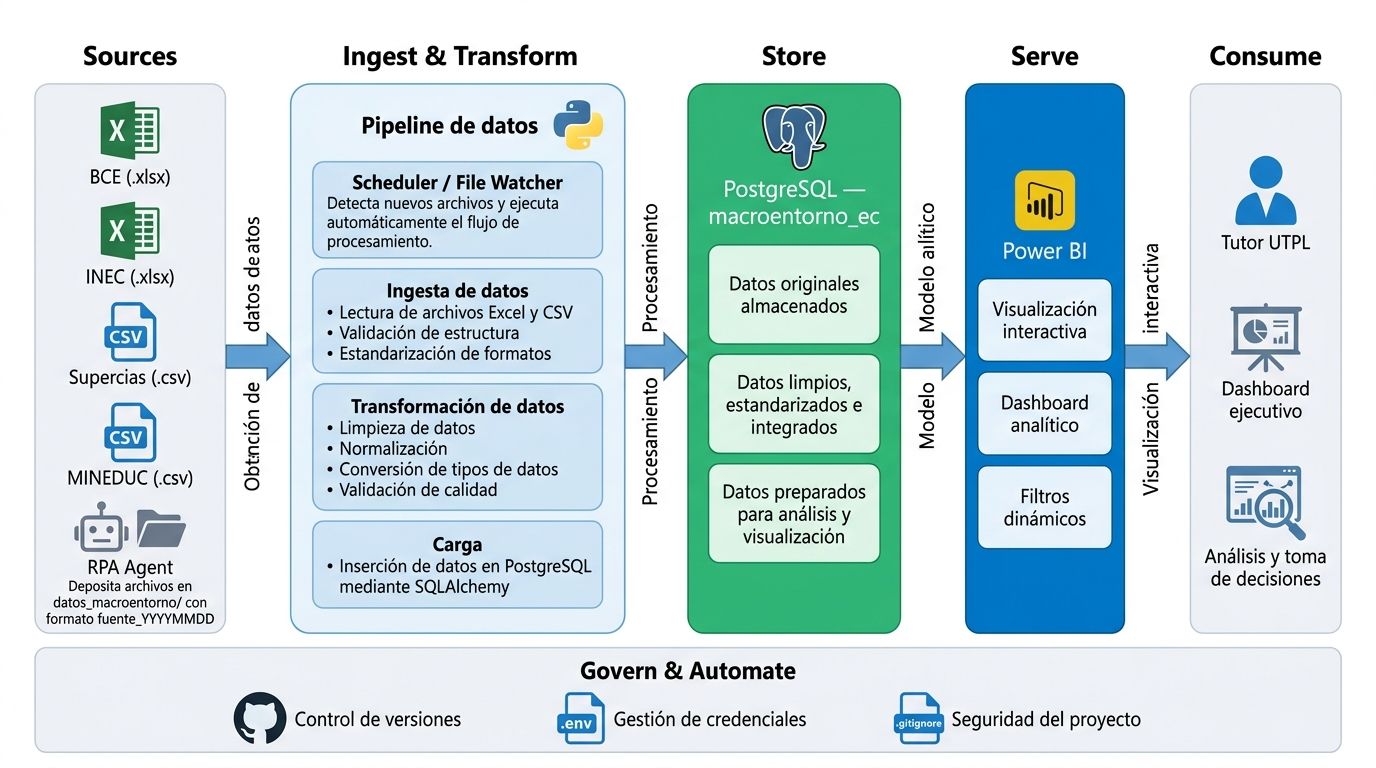
\includegraphics[width=\columnwidth]{arquitectura_pipeline.png}
  %%\imgplaceholder{Arquitectura Bronze-Silver-Gold con integracion RPA}{4.2cm}
  \caption{Arquitectura del pipeline del Macroentorno Ecuador.
    Almacena archivos crudos de RPA. Python transforma y carga
    en (PostgreSQL). Alimentan la visualizacion en Power~BI.}
  \label{fig:arquitectura}
\end{figure}

% =============================================================================
\begin{thebibliography}{13}

\bibitem{armbrust2021}
M.~Armbrust, A.~Ghodsi, R.~Xin y M.~Zaharia,
``Lakehouse: A new generation of open platforms that unify data
warehousing and advanced analytics,''
en \textit{Proc. 11th CIDR}, 2021.
\url{https://www.cidrdb.org/cidr2021/papers/cidr2021_paper17.pdf}

\bibitem{sawadogo2021}
P.~N.~Sawadogo y J.~Darmont,
``On data lake architectures and metadata management,''
\textit{J. Intell. Inf. Syst.}, vol.~56, no.~1, pp.~97--120, 2021.
\url{https://doi.org/10.1007/s10844-020-00608-7}

\bibitem{databricks2024}
Databricks,
``What is medallion lakehouse architecture?''
\textit{Microsoft Azure Docs}, 2024.
\url{https://learn.microsoft.com/en-us/azure/databricks/lakehouse/medallion}

\bibitem{jain2023}
P.~Jain, P.~Kraft, C.~Power, T.~Das, I.~Stoica y M.~Zaharia,
``Analyzing and comparing lakehouse storage systems,''
en \textit{Proc. 13th CIDR}, 2023.
\url{https://www.cidrdb.org/cidr2023/papers/p92-jain.pdf}

\bibitem{bhardwaj2024}
V.~Bhardwaj, A.~Noonia, S.~Chaurasia, M.~Kumar, A.~Rashid
y M.~T.~Ben~Othman,
``Optimizing structured data processing through robotic process
automation,''
\textit{J. Eur. Syst. Autom.}, vol.~57, no.~5, pp.~1523--1530, 2024.
\url{https://doi.org/10.18280/jesa.570528}

\bibitem{kimball2013}
R.~Kimball y M.~Ross,
\textit{The Data Warehouse Toolkit}, 3ra~ed.
Hoboken, NJ: John Wiley \& Sons, 2013.

\bibitem{barret2025}
N.~Barret et al.,
``Entity/Relationship graphs: Principled design, modeling, and data
integrity management,''
\textit{Proc. ACM Manag. Data}, vol.~3, no.~1, 2025.
\url{https://doi.org/10.1145/3709690}

\bibitem{machado2022}
I.~A.~Machado, C.~Costa y M.~Y.~Santos,
``Data mesh: Concepts and principles of a paradigm shift in data
architectures,''
\textit{Procedia Comput. Sci.}, vol.~196, pp.~263--271, 2022.
\url{https://doi.org/10.1016/j.procs.2021.12.033}

\bibitem{munappy2021}
A.~R.~Munappy, D.~I.~Mattos, J.~Bosch, H.~H.~Olsson y A.~Dakkak,
``From ad-hoc data analytics to DataOps,''
en \textit{Proc. IEEE ICSSP}, 2021.
\url{https://doi.org/10.1109/ICSSP52582.2021.00021}

\bibitem{naso2024}
J.~Naso y C.~Padden,
\textit{Data Platform Fundamentals}.
Dagster Labs, 2024.
\url{https://dagster.io/blog/data-platform-fundamentals}

\bibitem{lai2025}
E.~Lai, Y.~He y S.~Chaudhuri,
``Auto-Prep: Holistic prediction of data preparation steps for
self-service BI,''
\textit{Proc. VLDB Endow.}, vol.~14, no.~7, 2025.
arXiv:2504.11627.

\bibitem{tadakala2025}
L.~Tadakala et al.,
``Beyond visualization: Building decision intelligence through
iterative dashboard refinement,''
arXiv:2510.27572, 2025.
\url{https://arxiv.org/pdf/2510.27572}

\bibitem{wef2025}
World Economic Forum,
\textit{Future of Jobs Report 2025}.
Ginebra: WEF, 2025.
\url{https://www.weforum.org/publications/the-future-of-jobs-report-2025/}

\end{thebibliography}

\end{document}
